% Generated by pysimcount.pfmergesplit -- do not edit; regenerate instead.
% figure: merge-split-rz -- Childs et al. 2018 optimiser saving (Rz) split into exponential merging and optimiser-only, Suzuki formulas
% metric=rz gatebase=cz; n = 13, seed 1; r_method=emp (Eq. 147, as in Fig. 13); per-step counts, % of the unmerged simcount step
% optimised = Light reconstruction, marginal per step; verified n <= 13
% formulas: Lie-Trotter S1, Suzuki S2, Suzuki S4, Suzuki S6, Suzuki S8
% figure made at git_commit=e5d9ee696f892e28aced765585653760f8a427c4 git_dirty=False
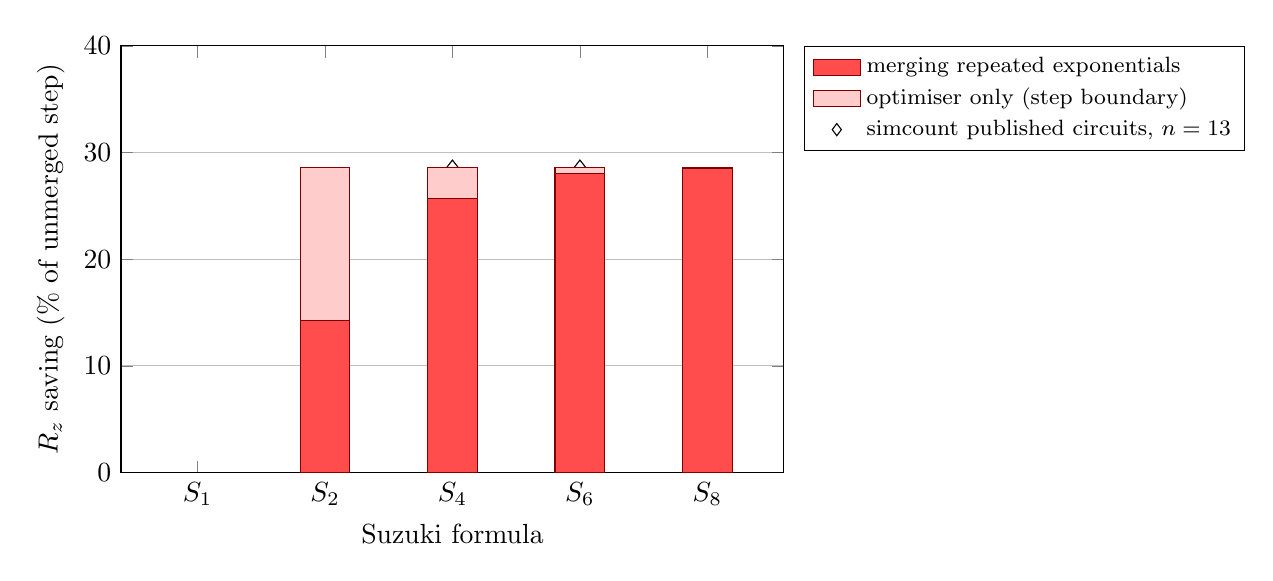
\begin{tikzpicture}
  \begin{axis}[
    width=10cm, height=7cm, ybar stacked, bar width=18pt,
    symbolic x coords={S1,S2,S4,S6,S8}, xtick=data,
    xticklabels={$S_1$,$S_2$,$S_4$,$S_6$,$S_8$},
    xlabel={Suzuki formula}, ylabel={$R_z$ saving (\% of unmerged step)},
    ymin=0, ymax=40, ymajorgrids=true, enlarge x limits=0.15,
    legend pos=outer north east, legend cell align=left, legend style={font=\footnotesize},
  ]
    \addplot[fill=red!70, draw=red!50!black, area legend] coordinates {
      (S1,0.0000)
      (S2,14.2857)
      (S4,25.7143)
      (S6,28.0000)
      (S8,28.4571)
    };
    \addlegendentry{merging repeated exponentials}
    \addplot[fill=red!20, draw=red!50!black, area legend] coordinates {
      (S1,0.0000)
      (S2,14.2857)
      (S4,2.8571)
      (S6,0.5714)
      (S8,0.1143)
    };
    \addlegendentry{optimiser only (step boundary)}
    \filldraw[draw=black, fill=white] (axis cs:S4,28.5583) ++(0pt,2.8pt) -- ++(2.2pt,-2.8pt) -- ++(-2.2pt,-2.8pt) -- ++(-2.2pt,2.8pt) -- cycle;
    \filldraw[draw=black, fill=white] (axis cs:S6,28.5604) ++(0pt,2.8pt) -- ++(2.2pt,-2.8pt) -- ++(-2.2pt,-2.8pt) -- ++(-2.2pt,2.8pt) -- cycle;
    \addlegendimage{line legend, only marks, mark=diamond*, mark size=2.2pt, mark options={draw=black, fill=white}}
    \addlegendentry{simcount published circuits, $n = 13$}
  \end{axis}
\end{tikzpicture}
